% !TEX TS-program = pdflatex
% !TEX encoding = UTF-8 Unicode

% This is a simple template for a LaTeX document using the "article" class.
% See "book", "report", "letter" for other types of document.

\documentclass[12pt,a4paper]{article} % use larger type; default would be 10pt

\usepackage[utf8x]{inputenc} % set input encoding (not needed with XeLaTeX)

%%% Examples of Article customizations
% These packages are optional, depending whether you want the features they provide.
% See the LaTeX Companion or other references for full information.

%%% PAGE DIMENSIONS
\usepackage{geometry} % to change the page dimensions
\geometry{a4paper} % or letterpaper (US) or a5paper or....
% \geometry{margin=2in} % for example, change the margins to 2 inches all round
% \geometry{landscape} % set up the page for landscape
%   read geometry.pdf for detailed page layout information

\usepackage{graphicx} % support the \includegraphics command and options
\usepackage{wrapfig}

% \usepackage[parfill]{parskip} % Activate to begin paragraphs with an empty line rather than an indent

%%% PACKAGES
\usepackage{booktabs} % for much better looking tables
\usepackage{array} % for better arrays (eg matrices) in maths
\usepackage{paralist} % very flexible & customisable lists (eg. enumerate/itemize, etc.)
\usepackage{verbatim} % adds environment for commenting out blocks of text & for better verbatim
\usepackage{subfig} % make it possible to include more than one captioned figure/table in a single float
% These packages are all incorporated in the memoir class to one degree or another...
\usepackage[ngerman]{babel}
\usepackage{pifont} %for symbols (i.e. arrows)

%%redifine of emph, see http://tex.stackexchange.com/questions/6754/what-is-the-canonical-way-to-redefine-the-emph-command
\makeatletter
\DeclareRobustCommand{\em}{%
  \@nomath\em \if b\expandafter\@car\f@series\@nil
  \normalfont \else \bfseries \fi}
\makeatother

%%% HEADERS & FOOTERS
\usepackage{fancyhdr} % This should be set AFTER setting up the page geometry
\pagestyle{fancy} % options: empty , plain , fancy
\renewcommand{\headrulewidth}{0pt} % customise the layout...
\lhead{}\chead{}\rhead{}
\lfoot{}\cfoot{\thepage}\rfoot{}

%%% SECTION TITLE APPEARANCE
\usepackage{sectsty}
\allsectionsfont{\sffamily\mdseries\upshape} % (See the fntguide.pdf for font help)
% (This matches ConTeXt defaults)

%%% ToC (table of contents) APPEARANCE
%\usepackage[nottoc,notlof,notlot]{tocbibind} % Put the bibliography in the ToC
%\usepackage[titles,subfigure]{tocloft} % Alter the style of the Table of Contents
%\renewcommand{\cftsecfont}{\rmfamily\mdseries\upshape}
%\renewcommand{\cftsecpagefont}{\rmfamily\mdseries\upshape} % No bold!

%%% END Article customizations

%%% The "real" document content comes below...

\title{Installation und Einrichtung von Microsoft Windows Server 2008 R2 zu einem Domain Controller}
\author{Sebastian Deußer}
%\date{} % Activate to display a given date or no date (if empty),
         % otherwise the current date is printed 
\setcounter{section}{-1}

\begin{document}
\maketitle %title (page)
\newpage
\tableofcontents
\newpage

\section{Installation von Windows Server 2008 R2}
Vor der Installation von Windows Server 2008 R2 sollte man erst einmal sicherstellen das man genug freien Platz auf der Festplatte hat, und diese wenn möglich schon einmal vorpartitionieren. Um noch etwas Luft zum arbeiten zu haben sollte man mindestens 30 GB reservieren.\\
Um die Installation nun zu starten legt man die Installations-DVD ins Laufwerk und bootet von dieser. Das Installationsprogramm ist selbsterklärend, man sollte aber darauf achten die richtige Partition als Installationsziel auszuwählen.\\
Wenn man einen anderen Bootloader als den von Windows verwendet (wie z.B. grub von Linux) muss man diesen nach der Installation wieder herstellen und einen Booteintrag für Windows Server 2008 R2.
\newpage

\section{Vorarbeiten}
Zunächst einmal sollte man dem Rechner der Domaincontroller werden soll einen Namen zuweisen. Dazu klickt man mit der rechten Maustaste auf \emph{Computer} und wählt \emph{Eigenschaften}. Hier wird der Computername angezeigt. Um ihn zu ändern klickt man die Schaltfläche \emph{Einstellungen ändern} (roter Kasten).

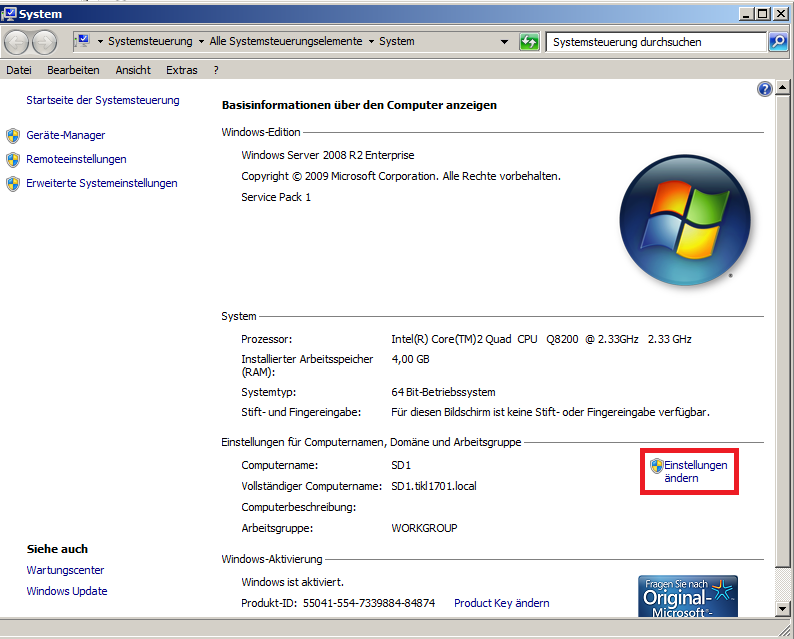
\includegraphics[width=14cm]{Bilder/001(Kasten)}\\
\newpage
Daraufhin erscheint folgender Dialog:

	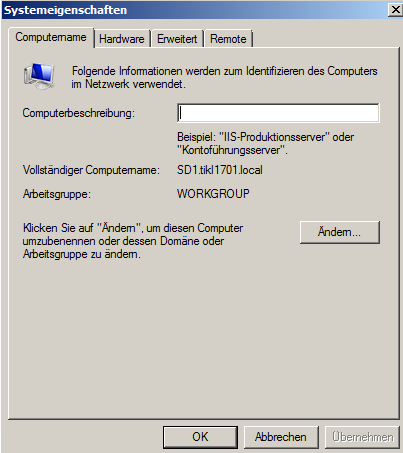
\includegraphics[width=8cm]{Bilder/002}
	
Hier kann man mit der Schaltfläche \emph{ändern} einen anderen Computernamen angeben.\\

	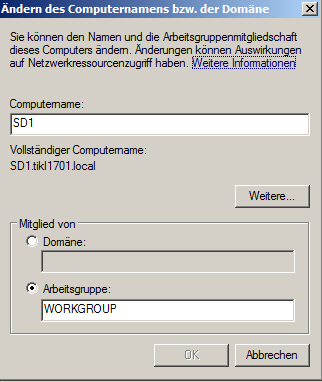
\includegraphics[width=8cm]{Bilder/003}
	
Die Arbeitsgruppe kann auf dem Standard belassen werden da dies eh angepasst wird bei der Installation des Domain Controllers.\\
Als nächstes muss man die IP-Einstellungen der Netzwerkkarte überprüfen, da ein Domain Controller eine feste IP benötigt. Die Einstellungen findet man z.B. unter \emph{Systemsteuerung \ding{221} Alle Systemsteuerungselemente \ding{221} Netzwerk- und Freigabecenter}, dort den Netzwerkadapter suchen und im rechte Maustasten Menü \emph{Eigenschaften} wählen. Dort \emph{Internetprotokoll Version 4 (TCP/IPv4)} auswählen und auf die Schaltfläche \emph{Eigenschaften} klicken.\\ %\ding{221} is one of the left arrows from pifont

	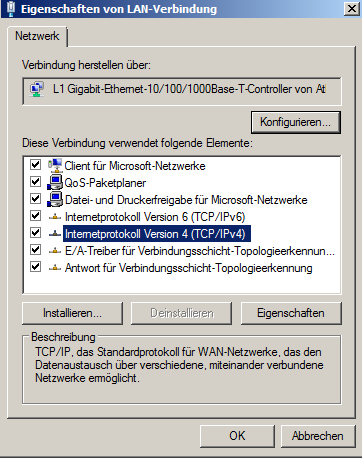
\includegraphics[width=8cm]{Bilder/004}\\
	
In dem folgenden Dialog kann man dann die IP-Adresse des Rechners fest. 

	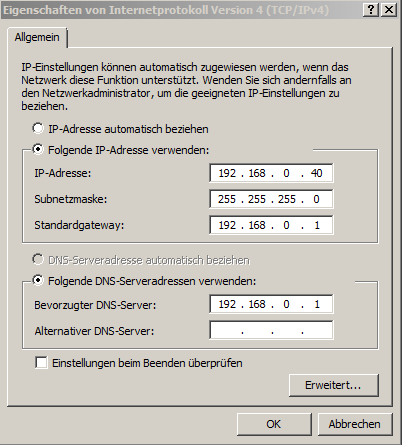
\includegraphics[width=8cm]{Bilder/005}\\
	
Dazu stellt man den Radiobutton auf \emph{Folgende IP-Adresse verwenden} und gibt dann eine in dem lokalen Netzwerk von keinem anderen Rechner benutzte IP-Adresse an, mit der passenden Subnetzmaske. als Standardgateway dient üblicherweise der Netzwerkrouter. Den DNS-Server muss man nun auch von Hand eingeben, dieser läuft üblicherweise auch auf dem Netzwerkrouter.\\
Damit wären die Vorarbeiten abgeschlosen, als nächstes wird die Active Directory-Domänendienste Rolle installiert.

\newpage
\section{Active Directory-Domänendienste installieren und einrichten}

\end{document}
